% SGA 3, Expose I, Loop 1 English reconstruction.
% Scope: Section 1.6 through the end of Remark 1.7.3.
% Authority: Polo--Gille Exp1-13oct24.pdf, component pages 5--10
% (combined-reader pages 15--20). OCR is drafting/locator material only.

\subsection*{1.6. Base change in a functor}

For every \(S\in\operatorname{Ob}(\mathscr C)\), there is a canonical functor
\[
  i_S:\mathscr C_{/S}\longrightarrow\mathscr C
\]
defined by \(i_S(f)=T\) when \(f\) is the arrow \(T\to S\). If
\(f:T\to S\) is an object of \(\mathscr C_{/S}\), we denote by
\(i_{T/S}=i_f\) the functor
\[
  i_{T/S}:(\mathscr C_{/S})_{/T}\longrightarrow\mathscr C_{/S},
\]
and there is a commutative diagram:

% Raster placeholder for Loop 1; replace by native TeX/TikZ in Loop 2.
% Authority: Exp1-13oct24.pdf p. 5; combined reader p. 15.
\begin{center}
  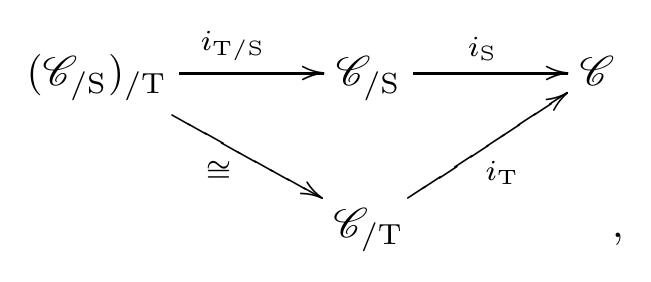
\includegraphics[width=0.57\textwidth]
    {figures/exp1/exp1_p005_base_change_triangle.png}
\end{center}

Thus, identifying \((\mathscr C_{/S})_{/T}\) with \(\mathscr C_{/T}\), as
we shall henceforth do,
\[
  i_S\circ i_{T/S}=i_T.
\]
Likewise, if \(\mathscr C\) is identified with \(\mathscr C_{/e}\) when
\(\mathscr C\) has a final object \(e\), then
\(i_{S/e}:\mathscr C_{/S}\to\mathscr C_{/e}\) is identified with \(i_S\).

For \(X\in\operatorname{Ob}(\mathscr C)\) (respectively,
\(Y\in\operatorname{Ob}(\mathscr C_{/S})\)), let \(p_S(X)\)
(respectively, \(p_{T/S}(Y)\)) be the object of \(\mathscr C_{/S}\)
(respectively, of \(\mathscr C_{/T}\)), when it exists, defined by
\(X\times S\) (respectively, \(Y\times_S T\)) equipped with its second
projection:

% Raster placeholder for Loop 1; replace by native TeX/TikZ in Loop 2.
% Authority: Exp1-13oct24.pdf p. 5; combined reader p. 15.
\begin{center}
  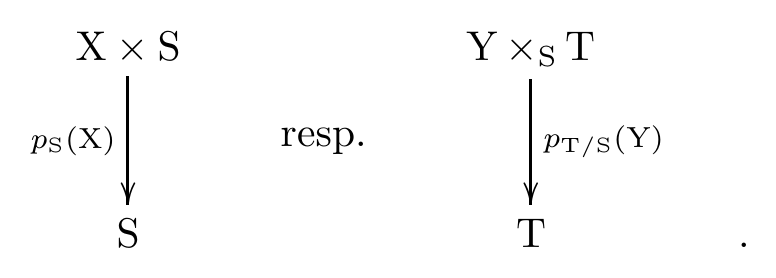
\includegraphics[width=0.62\textwidth]
    {figures/exp1/exp1_p005_base_change_projections.png}
\end{center}

The partially defined functor \(p_S\) (respectively, \(p_{T/S}\)) is called
the \emph{base-change functor}. By the definition of a product
(respectively, a fiber product), it is right adjoint to \(i_S\)
(respectively, to \(i_{T/S}\)).
\footnote{Editor's note: that is, if \(g:U\to S\) (respectively,
\(h:V\to T\)) is an object of \(\mathscr C_{/S}\) (respectively, of
\(\mathscr C_{/T}\)), then \(i_S(g)=U\), while \(i_{T/S}(h)\) is the
object \(f\circ h:V\to S\) of \(\mathscr C_{/S}\), and
\[
  \operatorname{Hom}_{\mathscr C_{/S}}(U,X\times S)
    \simeq \operatorname{Hom}_{\mathscr C}(U,X),
\]
respectively,
\[
  \operatorname{Hom}_{\mathscr C_{/T}}(V,X\times_S T)
    \simeq \operatorname{Hom}_{\mathscr C_{/S}}(V,X).
\]}
We also write
\[
  p_S(X)=X_S,
  \qquad
  p_{T/S}(Y)=Y_T.
\]

The functor \(i_S\) defines a restriction functor
\[
  i_S^*:\widehat{\mathscr C}\longrightarrow
    \widehat{\mathscr C_{/S}}.
\]
We write
\[
  \mathbf F_S=i_S^*(\mathbf F)=\mathbf F\circ i_S.
\]
Plainly,
\[
  i_{T/S}^*\circ i_S^*=i_T^*,
\]
that is, for every functor
\(\mathbf F\in\operatorname{Ob}(\widehat{\mathscr C})\),
\[
  (\mathbf F_S)_T=\mathbf F_T.
\]
The notation is justified by the following result.

\medskip
\noindent\textbf{Proposition 1.6.1.}
\textit{The functor
\[
  (\mathbf h_X)_S:(\mathscr C_{/S})^{\circ}\longrightarrow\mathbf{Set}
\]
is representable if and only if the product \(X\times S\) exists. In that
case
\[
  (\mathbf h_X)_S\simeq\mathbf h_{X_S}.
\]}

This shows that \(\mathbf F_S\) has two interpretations: it is the
restriction of \(\mathbf F\) to \(\mathscr C_{/S}\), and it is the functor
obtained by the base change \(e\leftarrow S\). This leads to the following
notation:

% Raster placeholder for Loop 1; replace by native TeX/TikZ in Loop 2.
% Authority: Exp1-13oct24.pdf p. 6; combined reader p. 16.
\begin{center}
  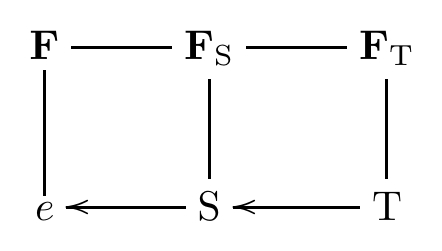
\includegraphics[width=0.38\textwidth]
    {figures/exp1/exp1_p006_functor_base_change_notation.png}
\end{center}

This diagram reflects both of the preceding interpretations. Notice that
\[
  \Gamma(\mathbf F_S)
    \simeq\operatorname{Hom}(\mathbf h_S,\mathbf F)
    \simeq\mathbf F(S),
\]
and, in particular,
\[
  \Gamma(X_S)\simeq\operatorname{Hom}(S,X).
\]

\subsection*{1.7.0.}

Let \(\mathbf E\) be an object of \(\widehat{\mathscr C}\).
\footnote{Editor's note: the lemma below has been added (see SGA~4,
I.3.4); it is used in the proof of 1.7.1 and will be useful repeatedly in
the sequel.}
Consider the category \(\mathscr C_{/\mathbf E}\) of \emph{objects of
\(\mathscr C\)} over \(\mathbf E\). Its objects are pairs \((V,\rho)\)
formed by an object \(V\) of \(\mathscr C\) and a morphism
\(\rho:\mathbf h_V\to\mathbf E\) in \(\widehat{\mathscr C}\), that is,
\(\rho\in\mathbf E(V)\). A morphism from \((V,\rho)\) to
\((V',\rho')\) is a morphism \(f:V\to V'\) in \(\mathscr C\) such that
\[
  \rho'\circ f=\rho,
  \qquad\text{that is,}\qquad
  \mathbf E(f)(\rho')=\rho.
\]
Let \(\mathbf L\) be the functor
\[
  \mathbf L=\varinjlim_{(V,\rho)\in\mathscr C_{/\mathbf E}}\mathbf h_V.
\]
Thus, for every \(S\in\operatorname{Ob}(\mathscr C)\),
\[
  \mathbf L(S)
    =\varinjlim_{(V,\rho)\in\mathscr C_{/\mathbf E}}\mathbf h_V(S)
\]
is the set of equivalence classes of triples \((V,\rho,v)\), where
\(v:S\to V\) is a morphism in \(\mathscr C\), and where
\((V,\rho,v)\) is identified with \((V',\rho',f\circ v)\) for every
morphism \(f:V\to V'\) in \(\mathscr C\) such that
\(\rho'\circ f=\rho\).

The map \(\phi_{\mathbf E}(S)\) which associates with the class of
\((V,\rho,v)\) the element \(\rho\circ v\) of \(\mathbf E(S)\) is well
defined and gives a morphism of functors
\[
  \phi_{\mathbf E}:
  \varinjlim_{(V,\rho)\in\mathscr C_{/\mathbf E}}\mathbf h_V
    \longrightarrow\mathbf E.
\]

\medskip
\noindent\textbf{Lemma.}
\textit{The morphism \(\phi_{\mathbf E}\) is an isomorphism.}

Indeed, let \(S\in\operatorname{Ob}(\mathscr C)\). Every
\(x\in\mathbf E(S)\) is the image under \(\phi_{\mathbf E}(S)\) of the
triple \((S,x,\operatorname{id}_S)\); hence \(\phi_{\mathbf E}(S)\) is
surjective. Conversely, let
\(\ell_1=(V_1,\rho_1,v_1)\) and
\(\ell_2=(V_2,\rho_2,v_2)\) be two elements of \(\mathbf L(S)\) having
the same image in \(\mathbf E(S)\), and set
\[
  \gamma=\rho_1\circ v_1=\rho_2\circ v_2.
\]
Then \(\ell_1\) and \(\ell_2\) are both equal in \(\mathbf L(S)\) to the
class of \((S,\gamma,\operatorname{id}_S)\). Thus
\(\phi_{\mathbf E}(S)\) is injective.

\medskip
\noindent\textbf{Corollary.}
\textit{For every object \(\mathbf F\) of \(\widehat{\mathscr C}\),
\[
  \operatorname{Hom}(\mathbf E,\mathbf F)
    =\varprojlim_{(V,\rho)\in\mathscr C_{/\mathbf E}}\mathbf F(V).
\]}

\subsection*{1.7. The objects \(\underline{\operatorname{Hom}}\),
\(\underline{\operatorname{Isom}}\), etc.}

Let \(\mathbf F\) and \(\mathbf G\) be two objects of
\(\widehat{\mathscr C}\). We define another object of
\(\widehat{\mathscr C}\) by
\begin{align*}
  \underline{\operatorname{Hom}}(\mathbf F,\mathbf G)(S)
  &={}\operatorname{Hom}_{\widehat{\mathscr C_{/S}}}
       (\mathbf F_S,\mathbf G_S)\\
  &\simeq\operatorname{Hom}_{\widehat{\mathscr C}_{/\mathbf h_S}}
       (\mathbf F\times\mathbf h_S,\mathbf G\times\mathbf h_S)\\
  &\simeq\operatorname{Hom}_{\widehat{\mathscr C}}
       (\mathbf F\times\mathbf h_S,\mathbf G).
\end{align*}
The object \(\underline{\operatorname{Hom}}(\mathbf F,\mathbf G)\) has
the following properties:
\begin{enumerate}
  \item[(i)]
    \(\underline{\operatorname{Hom}}(\underline{\mathbf e},\mathbf G)
      \simeq\mathbf G\).
    \footnote{Editor's note: if \(\mathbf E\) is a third object of
    \(\widehat{\mathscr C}\), then
    \[
      \underline{\operatorname{Hom}}(\mathbf E,\mathbf F\times\mathbf G)
      \simeq
      \underline{\operatorname{Hom}}(\mathbf E,\mathbf F)
        \times
      \underline{\operatorname{Hom}}(\mathbf E,\mathbf G).
    \]}
  \item[(ii)] The formation of \(\underline{\operatorname{Hom}}\) commutes
    with base extension:
    \[
      \underline{\operatorname{Hom}}(\mathbf F_S,\mathbf G_S)
        \simeq
      \underline{\operatorname{Hom}}(\mathbf F,\mathbf G)_S.
    \]
  \item[(iii)]
    \((\mathbf F,\mathbf G)\mapsto
      \underline{\operatorname{Hom}}(\mathbf F,\mathbf G)\)
    is a bifunctor, contravariant in \(\mathbf F\) and covariant in
    \(\mathbf G\).
\end{enumerate}
These three properties follow immediately from the definitions.

We shall prove that, for every object \(\mathbf E\) of
\(\widehat{\mathscr C}\),
\[
  \operatorname{Hom}
    \bigl(\mathbf E,
      \underline{\operatorname{Hom}}(\mathbf F,\mathbf G)\bigr)
    \simeq
  \operatorname{Hom}(\mathbf E\times\mathbf F,\mathbf G).
\]
Let \(\phi:\mathbf E\times\mathbf F\to\mathbf G\). We must associate
with it a morphism from \(\mathbf E\) to
\(\underline{\operatorname{Hom}}(\mathbf F,\mathbf G)\). For an arrow
\(S'\to S\) of \(\mathscr C\), there are maps
\[
  \mathbf E(S)\times\mathbf F(S')
    \longrightarrow
  \mathbf E(S')\times\mathbf F(S')
    \xrightarrow{\ \phi(S')\ }
  \mathbf G(S').
\]
Every element \(e\) of \(\mathbf E(S)\) therefore defines, for each
\(S'\to S\), a map \(\mathbf F(S')\to\mathbf G(S')\) functorial in
\(S'\); this is an element \(\theta_\phi(e)\) of
\(\underline{\operatorname{Hom}}(\mathbf F,\mathbf G)(S)\). We have thus
obtained a map
\[
  \phi\longmapsto\theta_\phi,
  \qquad
  \operatorname{Hom}(\mathbf E\times\mathbf F,\mathbf G)
    \longrightarrow
  \operatorname{Hom}
    \bigl(\mathbf E,
      \underline{\operatorname{Hom}}(\mathbf F,\mathbf G)\bigr),
\]
which is functorial in \(\mathbf E\).

\medskip
\noindent\textbf{Proposition 1.7.1.}
\footnote{Editor's note: part (b), which will be useful in II.1 and
II.3.11, has been added. A second, more direct proof of part (a) has also
been sketched.}
\textit{Let
\(\mathbf E,\mathbf F,\mathbf G\in
\operatorname{Ob}(\widehat{\mathscr C})\).
\begin{enumerate}
  \item[(a)] The map \(\phi\mapsto\theta_\phi\) is a bijection:
    \[
      \operatorname{Hom}(\mathbf E\times\mathbf F,\mathbf G)
        \xrightarrow{\ \sim\ }
      \operatorname{Hom}
        \bigl(\mathbf E,
          \underline{\operatorname{Hom}}(\mathbf F,\mathbf G)\bigr).
    \]
  \item[(b)] Moreover, there is an isomorphism of functors
    \[
      \underline{\operatorname{Hom}}
        \bigl(\mathbf E,
          \underline{\operatorname{Hom}}(\mathbf F,\mathbf G)\bigr)
        \simeq
      \underline{\operatorname{Hom}}
        (\mathbf E\times\mathbf F,\mathbf G).
    \]
\end{enumerate}}

For (a), regard both sides as functors of \(\mathbf E\). The asserted
result is true when \(\mathbf E=\mathbf h_X\), since it is then precisely
the definition of the functor
\(\underline{\operatorname{Hom}}(\mathbf F,\mathbf G)\). Moreover, both
sides, as functors of \(\mathbf E\), take direct limits to inverse limits.
Finally, by Lemma~1.7.0, every object \(\mathbf E\) of
\(\widehat{\mathscr C}\) is isomorphic to the direct limit of the
\(\mathbf h_X\), as \(X\) ranges over \(\mathscr C_{/\mathbf E}\). This
proves (a).

Let us also sketch a direct proof of (a). To every
\[
  \theta\in\operatorname{Hom}
    \bigl(\mathbf E,
      \underline{\operatorname{Hom}}(\mathbf F,\mathbf G)\bigr)
\]
associate \(\phi_\theta\in
\operatorname{Hom}(\mathbf E\times\mathbf F,\mathbf G)\) as follows. For
every \(S\in\operatorname{Ob}(\mathscr C)\), there is a map
\[
  \theta(S):\mathbf E(S)\longrightarrow
    \operatorname{Hom}(\mathbf F\times S,\mathbf G),
\]
functorial in \(S\). If
\((e,f)\in\mathbf E(S)\times\mathbf F(S)\), then \(f\) is a morphism
\(S\to\mathbf F\), so \(f\times\operatorname{id}_S\) is a morphism
\(S\to\mathbf F\times S\). On the other hand, \(\theta(S)(e)\) is a
morphism \(\mathbf F\times S\to\mathbf G\). Composition therefore gives
a morphism
\[
  \theta(S)(e)\circ(f\times\operatorname{id}_S):S\longrightarrow\mathbf G,
\]
that is, an element \(\phi_\theta(S)(e,f)\) of \(\mathbf G(S)\). It is
easy to check that \(S\mapsto\phi_\theta(S)\) is functorial in \(S\), and
therefore defines a morphism \(\phi_\theta\) from
\(\mathbf E\times\mathbf F\) to \(\mathbf G\). We leave to the reader the
verification that \(\theta\mapsto\phi_\theta\) and
\(\phi\mapsto\theta_\phi\) are mutually inverse bijections.

For (b), if \(S\in\operatorname{Ob}(\mathscr C)\), then by 1.7(ii) and
part (a), applied to \(\mathscr C_{/S}\),
\begin{align*}
  &\underline{\operatorname{Hom}}
    \bigl(\mathbf E,
      \underline{\operatorname{Hom}}(\mathbf F,\mathbf G)\bigr)(S)\\
  &\quad\simeq
    \operatorname{Hom}_S
      \bigl(\mathbf E_S,
        \underline{\operatorname{Hom}}_S(\mathbf F_S,\mathbf G_S)\bigr)\\
  &\quad\simeq
    \operatorname{Hom}_S
      (\mathbf E_S\times_S\mathbf F_S,\mathbf G_S)\\
  &\quad\simeq
    \operatorname{Hom}(\mathbf E\times\mathbf F\times S,\mathbf G)\\
  &\quad\simeq
    \underline{\operatorname{Hom}}
      (\mathbf E\times\mathbf F,\mathbf G)(S),
\end{align*}
and these isomorphisms are functorial in \(S\).

\medskip
\noindent\textbf{Corollary 1.7.2.}
\textit{There are isomorphisms
\[
  \operatorname{Hom}
    \bigl(\mathbf E,
      \underline{\operatorname{Hom}}(\mathbf F,\mathbf G)\bigr)
    \simeq
  \operatorname{Hom}
    \bigl(\mathbf F,
      \underline{\operatorname{Hom}}(\mathbf E,\mathbf G)\bigr),
\]
and
\[
  \underline{\operatorname{Hom}}
    \bigl(\mathbf E,
      \underline{\operatorname{Hom}}(\mathbf F,\mathbf G)\bigr)
    \simeq
  \underline{\operatorname{Hom}}
    \bigl(\mathbf F,
      \underline{\operatorname{Hom}}(\mathbf E,\mathbf G)\bigr).
\]}

In particular, taking \(\mathbf E=\underline{\mathbf e}\) and using
\(\underline{\operatorname{Hom}}(\underline{\mathbf e},\mathbf G)
\simeq\mathbf G\), we obtain
\[
  \Gamma\bigl(\underline{\operatorname{Hom}}(\mathbf F,\mathbf G)\bigr)
    \simeq\operatorname{Hom}(\mathbf F,\mathbf G).
\]
Composition supplies functorial morphisms
\[
  \underline{\operatorname{Hom}}(\mathbf F,\mathbf G)
    \times
  \underline{\operatorname{Hom}}(\mathbf G,\mathbf H)
    \longrightarrow
  \underline{\operatorname{Hom}}(\mathbf F,\mathbf H).
\]

If \(\mathbf F\) and \(\mathbf G\) are two objects of
\(\widehat{\mathscr C}\), let \(\operatorname{Isom}(\mathbf F,\mathbf G)\)
denote the subset of \(\operatorname{Hom}(\mathbf F,\mathbf G)\) formed by
the isomorphisms from \(\mathbf F\) onto \(\mathbf G\). Define a subobject
\(\underline{\operatorname{Isom}}(\mathbf F,\mathbf G)\) of
\(\underline{\operatorname{Hom}}(\mathbf F,\mathbf G)\) by
\[
  \underline{\operatorname{Isom}}(\mathbf F,\mathbf G)(S)
    =\operatorname{Isom}(\mathbf F_S,\mathbf G_S).
\]
Then
\[
  \Gamma\bigl(\underline{\operatorname{Isom}}
    (\mathbf F,\mathbf G)\bigr)
    \simeq\operatorname{Isom}(\mathbf F,\mathbf G),
  \qquad
  \underline{\operatorname{Isom}}(\mathbf F,\mathbf G)
    \simeq
  \underline{\operatorname{Isom}}(\mathbf G,\mathbf F).
\]
In the special case \(\mathbf F=\mathbf G\), set
\begin{align*}
  \underline{\operatorname{End}}(\mathbf F)
    &=\underline{\operatorname{Hom}}(\mathbf F,\mathbf F),
  &
  \operatorname{End}(\mathbf F)
    &=\operatorname{Hom}(\mathbf F,\mathbf F)
      \simeq\Gamma\bigl(\underline{\operatorname{End}}(\mathbf F)\bigr),\\
  \underline{\operatorname{Aut}}(\mathbf F)
    &=\underline{\operatorname{Isom}}(\mathbf F,\mathbf F),
  &
  \operatorname{Aut}(\mathbf F)
    &=\operatorname{Isom}(\mathbf F,\mathbf F)
      \simeq\Gamma\bigl(\underline{\operatorname{Aut}}(\mathbf F)\bigr).
\end{align*}
Formation of the objects
\(\underline{\operatorname{Hom}}\),
\(\underline{\operatorname{Isom}}\),
\(\underline{\operatorname{Aut}}\), and
\(\underline{\operatorname{End}}\) commutes with base change.

\medskip
\noindent\textbf{Remark 1.7.3.}
\footnote{Editor's note: the numbering 1.7.3 has been added for later
references.}
An object isomorphic to
\(\underline{\operatorname{Isom}}(\mathbf F,\mathbf G)\) may also be
constructed as follows. There is a morphism
\[
  \underline{\operatorname{Hom}}(\mathbf F,\mathbf G)
    \times
  \underline{\operatorname{Hom}}(\mathbf G,\mathbf F)
    \longrightarrow
  \underline{\operatorname{End}}(\mathbf F).
\]
Interchanging \(\mathbf F\) and \(\mathbf G\) gives a morphism
\[
  \underline{\operatorname{Hom}}(\mathbf F,\mathbf G)
    \times
  \underline{\operatorname{Hom}}(\mathbf G,\mathbf F)
    \longrightarrow
  \underline{\operatorname{End}}(\mathbf F)
    \times
  \underline{\operatorname{End}}(\mathbf G).
\]
On the other hand, the identity morphism of \(\mathbf F\) is an element of
\(\operatorname{End}(\mathbf F)\), and hence defines a morphism
\(\underline{\mathbf e}\to
\underline{\operatorname{End}}(\mathbf F)\). Doing the same for
\(\mathbf G\) and taking the product gives a morphism
\[
  \underline{\mathbf e}\longrightarrow
  \underline{\operatorname{End}}(\mathbf F)
    \times
  \underline{\operatorname{End}}(\mathbf G).
\]
It is then immediate that the fiber product of \(\underline{\mathbf e}\)
and
\[
  \underline{\operatorname{Hom}}(\mathbf F,\mathbf G)
    \times
  \underline{\operatorname{Hom}}(\mathbf G,\mathbf F)
\]
over
\(\underline{\operatorname{End}}(\mathbf F)
\times\underline{\operatorname{End}}(\mathbf G)\)
is isomorphic to
\(\underline{\operatorname{Isom}}(\mathbf F,\mathbf G)\).

All these definitions apply, in particular, when
\(\mathbf F=\mathbf h_X\) and \(\mathbf G=\mathbf h_Y\). If
\(\underline{\operatorname{Hom}}(\mathbf h_X,\mathbf h_Y)\) is
representable by an object of \(\mathscr C\), we denote that object by
\(\underline{\operatorname{Hom}}(X,Y)\). It has the following property:
if \(Z\times X\) exists, then
\[
  \operatorname{Hom}
    \bigl(Z,\underline{\operatorname{Hom}}(X,Y)\bigr)
    \simeq
  \operatorname{Hom}(Z\times X,Y).
\]
This property characterizes it when products exist in \(\mathscr C\).

Similarly, one defines, when they exist, the objects
\[
  \underline{\operatorname{Isom}}(X,Y),
  \qquad
  \underline{\operatorname{End}}(X),
  \qquad
  \underline{\operatorname{Aut}}(X).
\]
We merely note that the construction above shows that
\(\underline{\operatorname{Isom}}(X,Y)\) exists whenever fiber products
exist in \(\mathscr C\) and the objects
\[
  \underline{\operatorname{Hom}}(X,Y),
  \quad
  \underline{\operatorname{Hom}}(Y,X),
  \quad
  \underline{\operatorname{End}}(X),
  \quad\text{and}\quad
  \underline{\operatorname{End}}(Y)
\]
exist.

Everything above also applies to categories of the form \(\mathscr C_{/S}\).
The corresponding objects will be denoted as explicitly as possible by
appropriate symbols. For example, if \(T\) and \(T'\) are two objects of
\(\mathscr C\) over \(S\), we denote by
\(\underline{\operatorname{Hom}}_S(T,T')\) the object
\[
  \underline{\operatorname{Hom}}_{\mathscr C_{/S}}(T/S,T'/S).
\]

% End of assigned component. Section 1.8 begins in the next unit.
